\begin{frame}{La politique française}
  En groupes de 4, lisez ensemble le résumé de la politique française à la page 103 du manuel.
  Après le lire, répondez ensemble aux questions suivantes et discutez-en.
  \begin{columns}
    \column{0.4\textwidth}
      \begin{center}
        \href{https://www.youtube.com/watch?v=_3iEBJO2AV0}{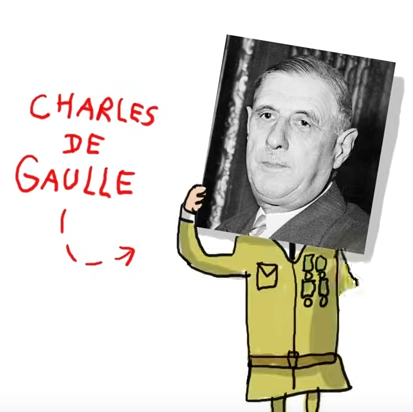
\includegraphics[scale=0.4]{de_gaulle.png}} \\
        \href{https://www.youtube.com/watch?v=ung6UiY3YY4}{L'Appel du 18 juin}
      \end{center}
    \column{0.6\textwidth}
      \begin{enumerate}
        \item Selon quels partis politiques est-ce que le gouvernement a un rôle à jouer dans la vie des citoyens?
        \item Quels problèmes les partis politiques doivent-ils résoudre?
        \item Qu'est-ce que la xénophobie? Quel parti est associé à la xénophobie? Imaginez les caractéristiques de ce parti. Un tel parti existe-t-il dans votre pays?
        \item Qu'est-ce que <<l'exception française>> à votre avis?
      \end{enumerate}
  \end{columns}
\end{frame}